\documentclass[a4paper]{article}

%% Language and font encodings
\usepackage[utf8]{inputenc}
\usepackage[T1]{fontenc}
\usepackage{fontspec}
\usepackage[ngerman]{babel}
% Bibliography for lua:
\usepackage[
backend=biber,
bibencoding=utf8
]{biblatex}
\addbibresource{Bibliothek.bib}

%\usepackage[numbers]{natbib} %definition for citation within the text (alternativ option: "numbers"
%\bibliographystyle{plain}
\usepackage{hyperref}

%% Sets page size and margins
\usepackage[a4paper,top=3cm,bottom=2.5cm,left=3.5cm,right=2.5cm,marginparwidth=1.75cm]{geometry}

%% Useful packages
\usepackage{amsmath}
\usepackage{graphicx}
\usepackage{xcolor}
\usepackage{tikz}
\usepackage{wrapfig}
\usepackage{xspace}

\definecolor{backg}{rgb}{0.85,0.85,0.85}

\usepackage{listings} % code formatting

\lstdefinestyle{my}{
    basicstyle = \small\ttfamily,
    keywordstyle=\ttfamily,
    language=bash,
    % morekeywords={
    % },
    backgroundcolor=\color{backg},
    numbers=left,
    commentstyle=\linespread{1.15}\footnotesize\color{olive},
    frame=tlbr, framesep=0.1cm
    }

\lstset{style=my}

\lstnewenvironment{mplisting}
{\newline\minipage[t]{\linewidth}}
{\endminipage \newline}

\newcommand{\inline}[1]{\colorbox{backg}{\lstinline{#1}}}
\usepackage{dirtree} 
\newcommand{\qq}[1]{\textit{\glqq#1\grqq}\xspace}

\makeatletter
\title{Versionskontrollsystem Git}\let\Title\@title
\author{Till Hanke}          \let\Author\@author
\date{\today}           \let\Date\@date
\makeatother



\begin{document}
\begin{titlepage}
	\centering
	{\scshape\LARGE Martin-Luther-Universität Halle-Wittenberg \par}
	\vspace{1cm}
	{\scshape\Large Bericht\par}
    zum Orientierungspraktikum\\
	\vspace{1.5cm}
	{\huge\bfseries \Title\par}
	\vspace{2cm}
    vorgelegt von\\
	{\scshape\Large \Author\par}
	\vfill
	\begin{flushleft}
    \begin{tabular}{llll}
    \textbf{Halle (Saale), den:} & & \Date &\\
    				& & \\
    \textbf{Betreuer:} & & Prof. Ingrid Mertig &\\
    \textbf{2. Gutachter:} & & PD Dr. Jürgen Henk &\\
    \end{tabular}
    \end{flushleft}
    % Bottom of the page
\end{titlepage}
\newpage
\tableofcontents
\newpage
\section{Einleitung}
Ein großer Teil der Forschung in der Physik umfasst das Schreiben und Entwickeln umfangreicher Programmcodes. Diese werden meist über Jahre oder gar Jahrzehnte hinweg aufgebaut. Viele Codes werden von großen Gruppen gemeinsam weiter entwickelt. Um einen Programmcode effizient zu dokumentieren und Änderungen auch Jahre später noch rückverfolgbar zu machen, wurden Versionskontrollsysteme genutzt. Diese Systeme sollen einen Überblick über den Verlauf von Änderungen verschaffen, aber auch die Zuordnung von Änderungen zu Autoren ermöglichen. Mittlerweile nutzen viele Entwickler Git als Versionskontrolle. Dafür werden zumeist auch öffentliche Server (\url{Gitlab.com} oder \url{Github.com}) genutzt, um den Code der Community zur Verfügung zu stellen\footnote{Auch der Quelltext dieser Arbeit steht auf Github zur Verfügung unter: {\url{https://github.com/tillhanke/Git-Einfuehrung}}}. 

Eine Bereitstellung von einem Quellcode sollte in wissenschaftlichen Arbeiten standardisiert werden. Git bietet genau solch einen Standard.

In diesem Bericht sollen Grundlagen der Arbeit mit Git erklärt werden. Der Fokus liegt dabei auf dem eigenständigen Arbeiten mit einer dezentralen Sicherung des Codes.

Alle Instruktionen in dieser Arbeit beziehen sich auf Linux Betriebssysteme. Die meisten der angegebenen Befehle werden auch auf MacOS Systemen funktionieren. Git ist ebenfalls für Windows OS verfügbar, was jedoch in diesem Bericht nicht betrachtet wird. Die Installation von Git auf den genutzten Maschinen wird vorausgesetzt.

Diese Arbeit orientiert sich maßgeblich an dem kostenlos verfügbaren Buch \cite{ProGit}, in dem Git sehr ausführlich erklärt wird. Für den interessierten Leser und die interessierte Leserin sind dort umfangreiche Erklärungen zu fortgeschrittenen Methoden nachzulesen.

\subsection{Versionskontrolle}
Das Ziel einer Versionskontrolle wie Git ist es, die Änderungen an einem Projekt zu dokumentieren. In Abb. \ref{fig:vers-kontrol}
ist eine solche Protokollierung visualisiert. Um Änderungen zu dokumentieren, werden zu jeder Änderung Kommentare hinzugefügt - sogenannte \qq{Commit-Messages}. Diese sollen ein späteres Zurückverfolgen der Änderungen vereinfachen. Um Speicherplatz zu sparen, werden in der Versionskontrolle möglichst nicht alle Dateien zu jedem Zeitpunkt gespeichert. Es wird nur einmal (zum Zeitpunkt der Erstellung) die komplette Datei gesichert. Danach werden von jeder Datei nur Informationen über die Änderungen abgespeichert.
\begin{figure}[!h]
    \centering
    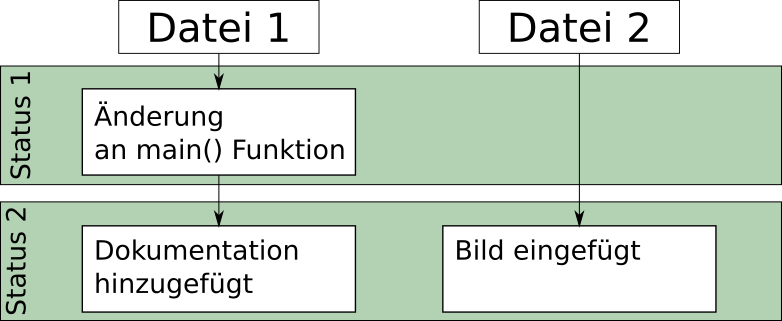
\includegraphics[width=0.9\textwidth]{Bilder/Versioncontrol.png}
    \caption{Beispiel einer Versionskontrolle von drei Änderungen an zwei Dateien desselben Projekts. Eingezeichnet sind zwei protokollierte Stadien des Projekts. Zu jeder Änderung ist ein Änderungskommentar angegeben.}
    \label{fig:vers-kontrol}
\end{figure}

\newpage
\section{Initialisierung eines lokalen .git}
Git muss in dem Hauptordner eines Projekts initialisiert werden. Das bedeutet, dass alle Projekt-Dateien in Unterordnern zu finden sein müssen (eine exemplarische Ordnerstruktur ist in \ref{fig:dir_struc} dargestellt). Bei der Initialisierung von Git wird im Hauptordner zusätzlich ein neuer Unterordner  \inline{.git/} angelegt. In diesem Ordner wird Git alle Versionsinformationen und die Historie abspeichern. Durch Löschen des Ordners wird Git von dem Projekt getrennt.
\begin{figure}[!h]
    \dirtree{%
    .1 Git-Basics.
    .2 .git.
    .3 \ldots \hspace{2ex}\begin{minipage}[t]{8cm}In diesem Ordner werden die Informationen über Änderungen abgespeichert\end{minipage}.
    .2 Bilder.
    .3 git\_commit.png.
    .3 Versioncontrol.png.
    .2 main.tex.
    .2 Title.tex.
    .2 initialisierung.tex.
    .2 Einleitung.tex.
    .2 Commit.tex.
    .2 Bibliothek.tex.
    }
    \caption{Exemplarische Ordnerstruktur für ein Projekt mit Git.}
    \label{fig:dir_struc}
\end{figure}

Um in einem Projektordner Git zu initialisieren, genügt der Befehl. 
\begin{mplisting}
$ git init
\end{mplisting}
Dadurch wird in dem aktuellen Verzeichnis ein \inline{.git} Ordner angelegt.
%
\subsection{Git Config}
Um Änderungen zu protokollieren, benötigt Git Informationen über den User. Diese Informationen können System-übergreifend pro User oder für das jeweilige Projekt hinterlegt werden. Die benötigten Informationen sind eine Email-Adresse und ein Benutzername. Definiert werden die Informationen mithilfe von \inline{git config}. Durch die Angabe einer Option wird definiert, ob diese Information für das System (\inline{--system}), den User (\inline{--global}) oder das Projekt (\inline{--local}) abgespeichert werden sollen.
\begin{lstlisting}[breaklines=true]
$ git config --global user.name "Max Mustermann"
$ git config --global user.email "max@mustermann.de"
$ git config --global core.editor vim  # Dieser Editor wird von git genutzt um Eingaben des Users ab zu fragen.
\end{lstlisting}
Nach der Initialisierung kann der Status des Git mit \inline{git status} abgefragt werden.
\begin{mplisting}
$ ls -a
.   Bibliothek.bib  Commit.tex      .git                 main.tex
..  Bilder          Einleitung.tex  initialisierung.tex  Title.tex
$ git status
On branch master

No commits yet

Untracked files:
  (use "git add <file>..." to include in what will be committed)
	Bibliothek.bib
	Bilder/
	Commit.tex
	Einleitung.tex
	Title.tex
	initialisierung.tex
	main.tex

nothing added to commit but untracked files present (use "git add" to track)

\end{mplisting}
Durch diese Initialisierung wird ein leeres Git-Repository angelegt. 
Es ist zu erkennen, dass alle Dateien des Projektes als \qq{untracked} erkannt wurden. Dies ist einer von 4 verschiedenen Zuständen, in die Git Dateien sortiert. Eine Übersicht der 4 Zustände ist in Abb. \ref{fig:lifecycle} dargestellt.
\begin{figure}[!h]
	\centering
	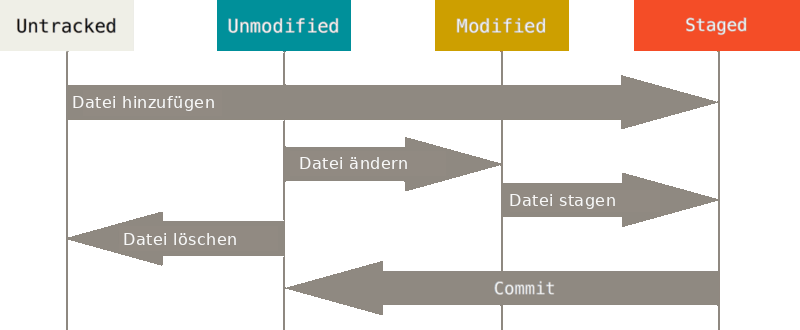
\includegraphics[width=\textwidth]{Bilder/lifecycle_de.png}
	\caption{Die 4 Zustände, in denen eine Datei sich im Git befinden kann. Die Pfeile geben an, wie die Dateien zwischen den Stadien wechseln. Das Bild wurde aus \cite{ProGit} entnommen und leicht verändert.}
	\label{fig:lifecycle}
\end{figure}

Um Änderungen von Dateien zu protokollieren, müssen die gewünschten Dateien auf \qq{staged} gesetzt werden. Das geschieht mithilfe des   \inline{git add} Befehls.
\begin{mplisting}
$ git add main.tex
$ git status
On branch master

No commits yet

Changes to be committed:
  (use "git rm --cached <file>..." to unstage)
	new file:   main.tex

Untracked files:
  (use "git add <file>..." to include in what will be committed)
	Bibliothek.bib
	Bilder/
	Commit.tex
	Einleitung.tex
	Title.tex
	initialisierung.tex
\end{mplisting}
\inline{git status} zeigt direkt, wie man Dateien wieder \qq{unstaged} setzen kann. Als nächstes sollen jedoch alle Dateien, die \qq{untracked} sind \qq{staged} werden. Damit wir nicht alle Dateien einzeln aufrufen müssen, kann der gesamte Projektordner \qq{staged} gesetzt werden:
\begin{mplisting}
$ git add .
$ git status
On branch master

No commits yet

Changes to be committed:
  (use "git rm --cached <file>..." to unstage)
	new file:   Bibliothek.bib
	new file:   Bilder/Versioncontrol.png
	new file:   Bilder/git_commit.png
	new file:   Commit.tex
	new file:   Einleitung.tex
	new file:   Title.tex
	new file:   initialisierung.tex
	new file:   main.tex

\end{mplisting}
Damit wurden alle Dateien \qq{gestaged}. Noch hat Git die Änderungen nicht protokolliert, sondern nur die Dateien markiert um sie bei dem nächsten Commit zu protokollieren. Dateien, die keine unprotokollierten Änderungen haben befinden sich im Status \qq{unmodified}. Alle \qq{staged} Dateien werden durch den Commit in \qq{unmodified} überführt.
%
\newpage
\section{Erster Commit}
\begin{lstlisting}
$ git add README.md
$ git status
On branch master

No commits yet

Changes to be committed:
  (use "git rm --cached <file>..." to unstage)
        new file:   README.md
\end{lstlisting}
An dieser Stelle wurde die Datei
\inline{README.md} dem nächsten Commit hinzugefügt. Um den Aktuellen Status zu protokollieren muss der Befehl \inline{git commit} genutzt werden. Dabei werden alle Änderungen Protokolliert.
Git speichert intern die Version der Datei ab und verweißt in jedem folge Commit darauf. Wenn die Datei nicht verändert wird wird somit nicht mehr Speicherplatz verwendet, egal in wie vielen Commits die Datei vorkommt.
Ein commit wird immer mit einer Commit-Message begleitet. Wenn der Befehl \inline{git commit} ohne Optionen ausgeführt wird öffnet sich daher automatisch der standard editor (der über \inline{git config --local core.editor} definiert wurde). In diesem Befindet sich eine auskommentierte Übersicht des Commits. Darunter muss eine Commit-Message eingefügt werden.
\begin{figure}[!h]
        \centering
        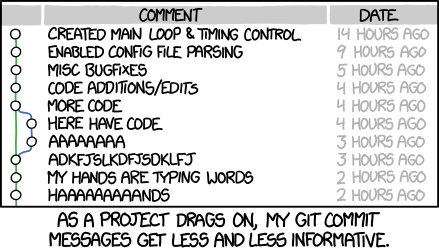
\includegraphics[width=0.5\textwidth]{Bilder/git_commit.png}
        \caption{Eine Commitbaum-Darstellung von XKCD \cite{Munroe}. Die Commit-Messages starten oben mit den ersten Commits sehr vorbildlich. Nach einigen Commits ist zu sehen, dass die Messages keine informationen über den Commit Inhalt mehr haben. Dies ist ein häufiges Problem, wenn zu selten Committed wird kann es schnell passieren, dass nicht mehr klar ist, was sich seit dem letzten Commit alles geändert hat. Dadurch werden Commit-Messages schnell schwer zu schreiben und vernachlässigt.}
        \label{fig:commit-XKCD}
\end{figure}

Commit-Messages sollten 
%
\newpage
\section{Branches}\label{sec:branch}
Während der Entwicklung eines Programms ist es meist nützlich mehrere Versionen parallel zu verwalten. Das kann heißen, dass es eine \qq{release} Version und eine \qq{developement} Version gibt oder, dass man die letzte funktionierende Variante des Programms erhalten will während man neue Funktionen versucht zu implementieren.

Die parallele Entwicklung an mehreren Versionen wird durch Branches ermöglicht.
\subsection{Branch erstellen}
Um einen Branch zu erstellen wird \inline{git branch [Name]}, mit einem Namen für den Branch, genutzt. Mit \inline{git checkout} wird der aktive Branch ausgewählt. Der Log zeigt den Verlauf, des gerade aktiven Branches an.
\begin{mplisting}
$ git branch section4
$ git checkout section4
$ git log --pretty=format:"%h %s %d"
04965ab add: sentence at end of Commit  (HEAD -> section4, master)
906a721 add: label for future sections 
03a1fee add: Subsection about reverting commits 
bf11cfe add: files to ignore from macOS 
\end{mplisting}
Hier kann man sehen, dass sowohl \inline{master}, als auch \inline{section4} auf denselben Commit zeigen (\inline{04965ab}). Jeder neue Commit jedoch wird nur von dem Branch erfasst, auf den \inline{HEAD} zeigt (\inline{section4}).

\begin{figure}[!h]
	\centering
	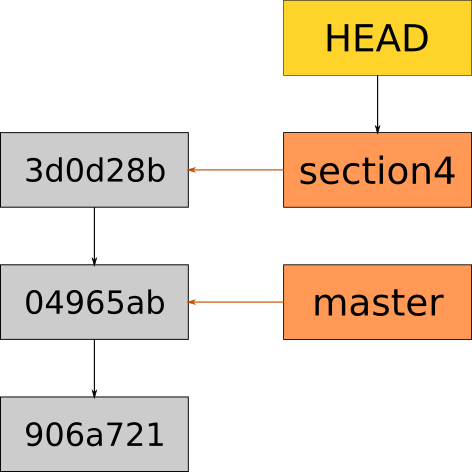
\includegraphics[width=0.4\textwidth]{Bilder/branching.png}
	\caption{Beispielhafter Commit-Baum aus diesem Projekt. Graue Kästen stellen einzelne Commits dar, orangene Branches und der gelbe Kasten ist der aktuelle HEAD. Die Pfeile zeigen auf die Verlinkung.}
	\label{fig:branch_1}
\end{figure}
Abb. \ref{fig:branch_1} zeigt den Commit-Baum des Repositories nach dem ersten Commit in \inline{section4}. \inline{HEAD} zeigt auf den aktuellen Zustand des lokalen Ordners. In diesem Fall auf den Branch \inline{section4}. Die Branches selber zeigen auf den Commit, den sie gerade darstellen. Um den \inline{HEAD} zu wechseln muss nur \inline{git checkout [BRANCH]} mit dem entsprechenden Branch aufgerufen werden.
\begin{figure}[!h]
	\centering
	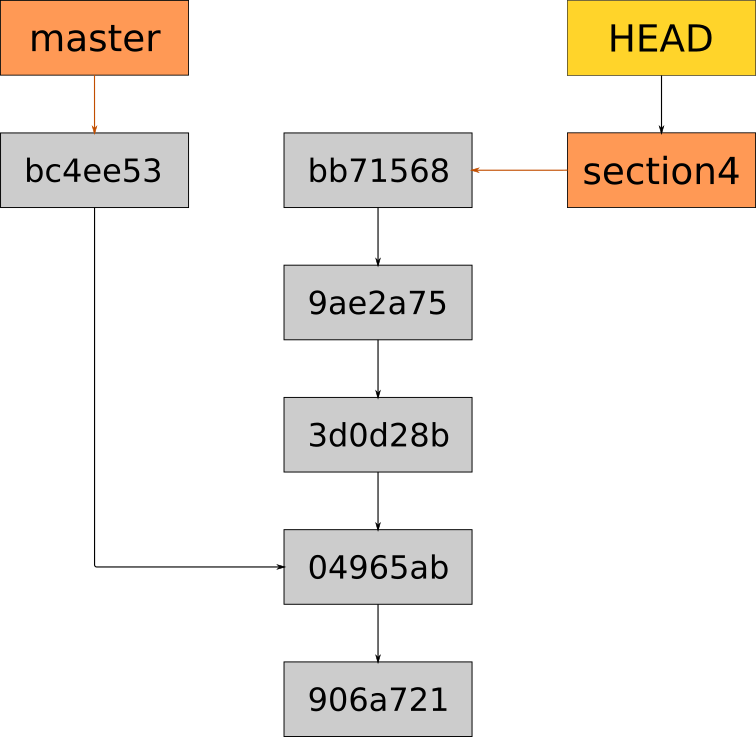
\includegraphics[width=0.4\textwidth]{Bilder/branching_2.png}
	\caption{Branch-tree nachdem mehrere Commits zu den Branches gemacht wurden.}
	\label{fig:branch_2}
\end{figure}

\subsection{Merging}
Das Zusammenführen zweier Branches wird Merging genannt. Dabei ist das Ziel, alle Änderungen der beiden Branches zu vereinen. Wichtig ist, dass immer der Branch ausgewählt (\inline{HEAD} zeigt darauf) sein sollte, in dem die Änderungen vereint werden sollen. Will man also in \inline{master} die Änderungen von \inline{section4} einbinden geht das folgendermaßen:
\begin{mplisting}
$ git checkout master
$ git merge section4
Merge made by the 'recursive' strategy.
Bilder/branching.png   | Bin 0 -> 25763 bytes
Bilder/branching.svg   | 648 +++++++++++++++++++++++++++++++++++
Bilder/branching_2.png | Bin 0 -> 41671 bytes
branches.tex           |  36 +++++
main.tex               |   3 +-
5 files changed, 686 insertions(+), 1 deletion(-)
create mode 100644 Bilder/branching.png
create mode 100644 Bilder/branching.svg
create mode 100644 Bilder/branching_2.png
create mode 100644 branches.tex
\end{mplisting}
Durch das mergen wird ein neuer Commit angelegt, welcher auf beide  \qq{parents} verweist (vgl. Abschnitt \ref{sec:first_commit}, statt einem \qq{parent} hat dieser Commit zwei). Nachdem ein Branch gemerged wurde kann er gelöscht werden.
\begin{figure}[!ht]
	\centering
	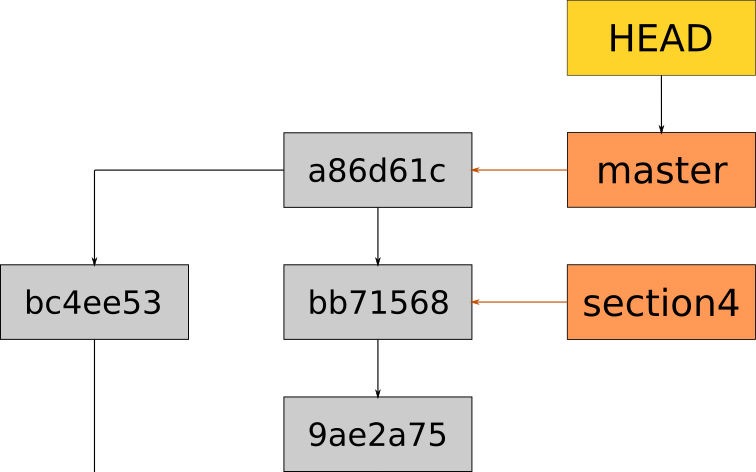
\includegraphics[width=0.6\textwidth]{Bilder/branching_3.png}
	\caption{Commit-Baum nach dem Merging. Der Merge wird als eigener Commit oberhalb der beiden \qq{parent}-Commits angezeigt. Der \inline{master} Branch und \inline{HEAD} zeigen beide auf den Merge-Commit. Der \inline{section4} Branch existiert weiterhin, zeigt jedoch auf den alten Commit.}
	\label{fig:merge}
\end{figure}

% MERGE Conflicts missing
% - mergeconflicts not yet included
%
\newpage
\section{Remotes}
Ein Git kann nicht nur lokal geführt werden. Wirklich effektiv werden Gits wenn man sie mit einem remote-Server verbindet. Dieser Server kann auf verschiedenste Arten erreichbar sein. Die häufigsten Methoden einen remote-Server an zu sprechen sind jedoch http(s) und ssh. 
\subsection{Github}
Es gibt online verschiedene Anbieter für Git-Server. \url{Github.com} ist einer der wohl bekanntesten. Um ein Projekt bei Github zu veröffentlichen (oder privat dort zu sichern) muss ein Benutzeraccount angelegt werden.

In diesem Beispiel wird gezeigt, wie man ein lokales Git per SSH auf Github synchronisieren kann. Um ssh mit Github zu verwenden muss ein SSH-Key auf dem lokalen PC erstellt werden, und der öffentliche Schlüssel bei Github hinterlegt werden. Ein SSH-Key kann mit \inline{ssh-keygen} erzeugt werden. Als Standard wird dadurch ein RSA Key-Paar erzeugt und im \inline{/home/user/.ssh/} Ordner hinterlegt.
Es entstehen in diesem Ordner \inline{id_rsa} und \inline{id_rsa.pub} die Datei, die mit .pub endet enthält den öffentlichen Schlüssel, der weitergegeben werden kann. Die andere Datei sollte niemals weitergegeben werden. Sie enthält den privaten Schlüssel, mit dem man sich dann authentifizieren kann.
\begin{mplisting}
$ ssh-keygen  # erzeugen eines Schlüsselpaares
$ cat ~/.ssh/id_rsa.pub  # anzeigen des öffentlichen Schlüssels
ssh-rsa
AAAAB3NzaC1yc2EAAAADAQABAAABgQDMuksDJfybOInEWtN+tSxLmjT/wG5q6ZY4aZFRB
lhoho865XwJZZm1DAdL0Ec9Lt1DfHfAhX9QOTlJW1qXX6dn1dtD5ih6n41tdxpxxJ/P2a
6YHGGKYQ0p7qSqzS5ydu+GST73lWxK8eDrU8Tm+lDRpyGu4GRqph5gemFyzW11AD2OknW
cm+Zp9ghHWUZuGGH8KqYWAHjkMDuZZMchC4f7IhrVZwhiiWFMyS7BEaIb8FrKtpTnjeoH
4qkaHNr8umFxatZRLYqHMrx/JA0/4JwLFNOtZTVTl220Nst5+cCx54ZhDHi1AeROMZ5xw
BPiYHi3eBsEfHZBt6euJNWcdVoq6bZK+ImXA1IszqevJNu571g9sBHjOtkgrXVoYVicnC
wGYI2Fnd4VRjPV+4xSLnizqr0fMvXlGdTvlyXML4gA+eyYwBF83xQ35F2e8FA+dGCzyGL
7A/zd1yDh1jVgsiQMVwuA3xVEGWnVzo6kXk/qCuMaIivLi3R9vuokdwL+iak= till@phys-87
\end{mplisting}
Dieser öffentliche Schlüssel kann nun bei Github unter \inline{settings -> SSH and GPG keys -> New SSH key} eingegeben werden. Damit kann man von dem Rechner aus, auf dem der Schlüssel erzeugt wurde, auf jedes Github Repository des Benutzeraccounts zugreifen.

\subsection{Remote hinzufügen}
Mit \inline{git remote} kann man alle verknüpften Remotes auflisten lassen. Um ein Github Repository als Remote mit dem lokalen Git zu verknüpfen muss zuerst ein Github Repository online erstellt werden. Diesem neuen Repository muss ein Name gegeben werden, nach der Erstellung kann das lokale Repository mit Github verbunden werden.
\begin{mplisting}
$ git remote add github git@github.com:[Benutzername]/[Github Projektname].git
$ git remote
\end{mplisting} 
Dabei muss dem remote ein Name gegeben werden (hier \inline{github}) und der Link zu dem remote Repository angegeben werden (bestehend aus dem Benutzername und dem Namen des Github Repository). \inline{git remote} sollte daraufhin den Namen des gerade hinzugefügten remotes auflisten (\inline{github}). Damit ist das lokale Repository jedoch noch nicht auf Github zu sehen. Um den aktuellen Stand des lokalen Repositories zu Github zu pushen muss \inline{git push} genutzt werden.
\begin{mplisting}
$ git push github master
\end{mplisting}
\inline{git push} benötigt mindestens zwei Argumente. Das erste Argument gibt den remote an zu dem gepushed werden soll (es können mit einem lokalen Repository mehrere remotes verbunden werden) das zweite Argument gibt den Branch an, der gepushed werden soll. Durch diesen Befehl wird der lokale Branch mit dem remote Branch gemerged. Falls das remote Repository diesen Branch noch nicht hat wird dieser erzeugt.
% - ssh custom server remote
% - gitlab/github with https
%
\newpage
\section{Zusammenfassung}
In dieser Arbeit wurde auf die Grundlagen der Nutzung von Git eingegangen. Dabei wurde gezeigt, wie man lokale Repositories anlegen kann. Wie die Arbeit lokal verfolgt wird, und wie man parallel an verschiedenen Versionen Arbeiten kann.

Zusätzlich wurde die Nutzung von sogenannten Remotes (entfernten Github Repositories) dargestellt um die eigene Arbeit zu sichern oder mit anderen Entwicklern (oder Nutzern) zu teilen. Diese Arbeit stellt keinerlei Anspruch an Vollständigkeit, sondern soll nur den Einstieg in die Arbeit mit Git ermöglichen.

Für weiterführende Informationen soll noch einmal das Buch \cite{ProGit} empfohlen werden, welches online zur freien Verfügung steht und alle hier aufgeführten Themen (und noch viele mehr) in tieferem Detail bespricht.
\newpage
\nocite{*}

\printbibliography

\end{document}